\subsection{DC Supplies} \label{subsec:DCSupples}

Several DC supplies are required to power the impedance analyzer, so an overview has been made to visualize this in table \refq{tab:7_1_6_Supply_Voltages}.
\begin{table}[ht]
\centering
\begin{tabular}{@{}ll@{}}
\toprule
\textbf{Category}       & \textbf{Details}                                                                                 \\ \midrule
\textbf{Analog circuits} &                                                                                                 \\
\quad +6V                & For ADC Buffers                                                                                \\
\quad -1V                & For ADC Buffers                                                                                \\
\quad +5V                & For ADC and DAC, Anti-Aliasing Filters, DAC Reconstruction Filters                                                                                  \\
\quad -5V                & DAC, Anti-Aliasing Filters, DAC Reconstruction Filters  \\
\quad +2.5V              & For ADC digital interface                                                                      \\
\quad $\pm$12V           & Programmable Amplifiers, DAC Output Power Amplifier, Range Relays               \\
                         &                                                        \\ \midrule
\textbf{Digital circuits} &                                                                                                 \\
\quad +5V                & For Artix 7 Development Board, STM32 Nucleo Development Board,                                 \\
                         & and Nextion Touchscreen                                                                        \\ \bottomrule
\end{tabular}
\caption{Overview of Supply Voltages in the System}
\label{tab:7_1_6_Supply_Voltages}
\end{table}

An estimate of the expected load is required in order to make the DC supplies from table \refq{tab:7_1_6_Supply_Voltages}. This estimate has been made and can be seen in appendix \refq{App:PowerConsumption}. A Mean Well RT65C\cite{RT65C} power supply will be used to power the impedance analyzer, it will supply a $\pm 15V$ rail a long with a $+5V$ rail. The $+5V$ rail will be used to power the digital circuits directly, while the $\pm 15V$ will be used to power the analog front end. The analog supplies will be kept separate from the digital supply to reduce noise in the analog circuits.

$\pm 15V$ supply from the RT65C is regulated to supplies listed in table \refq{tab:7_1_6_Supply_Voltages} with several linear voltage regulators as shown in the diagram for the supply on figure \refq{fig_7_1_6_DCSUPPLY}.

\begin{figure}[H]
    \centering
    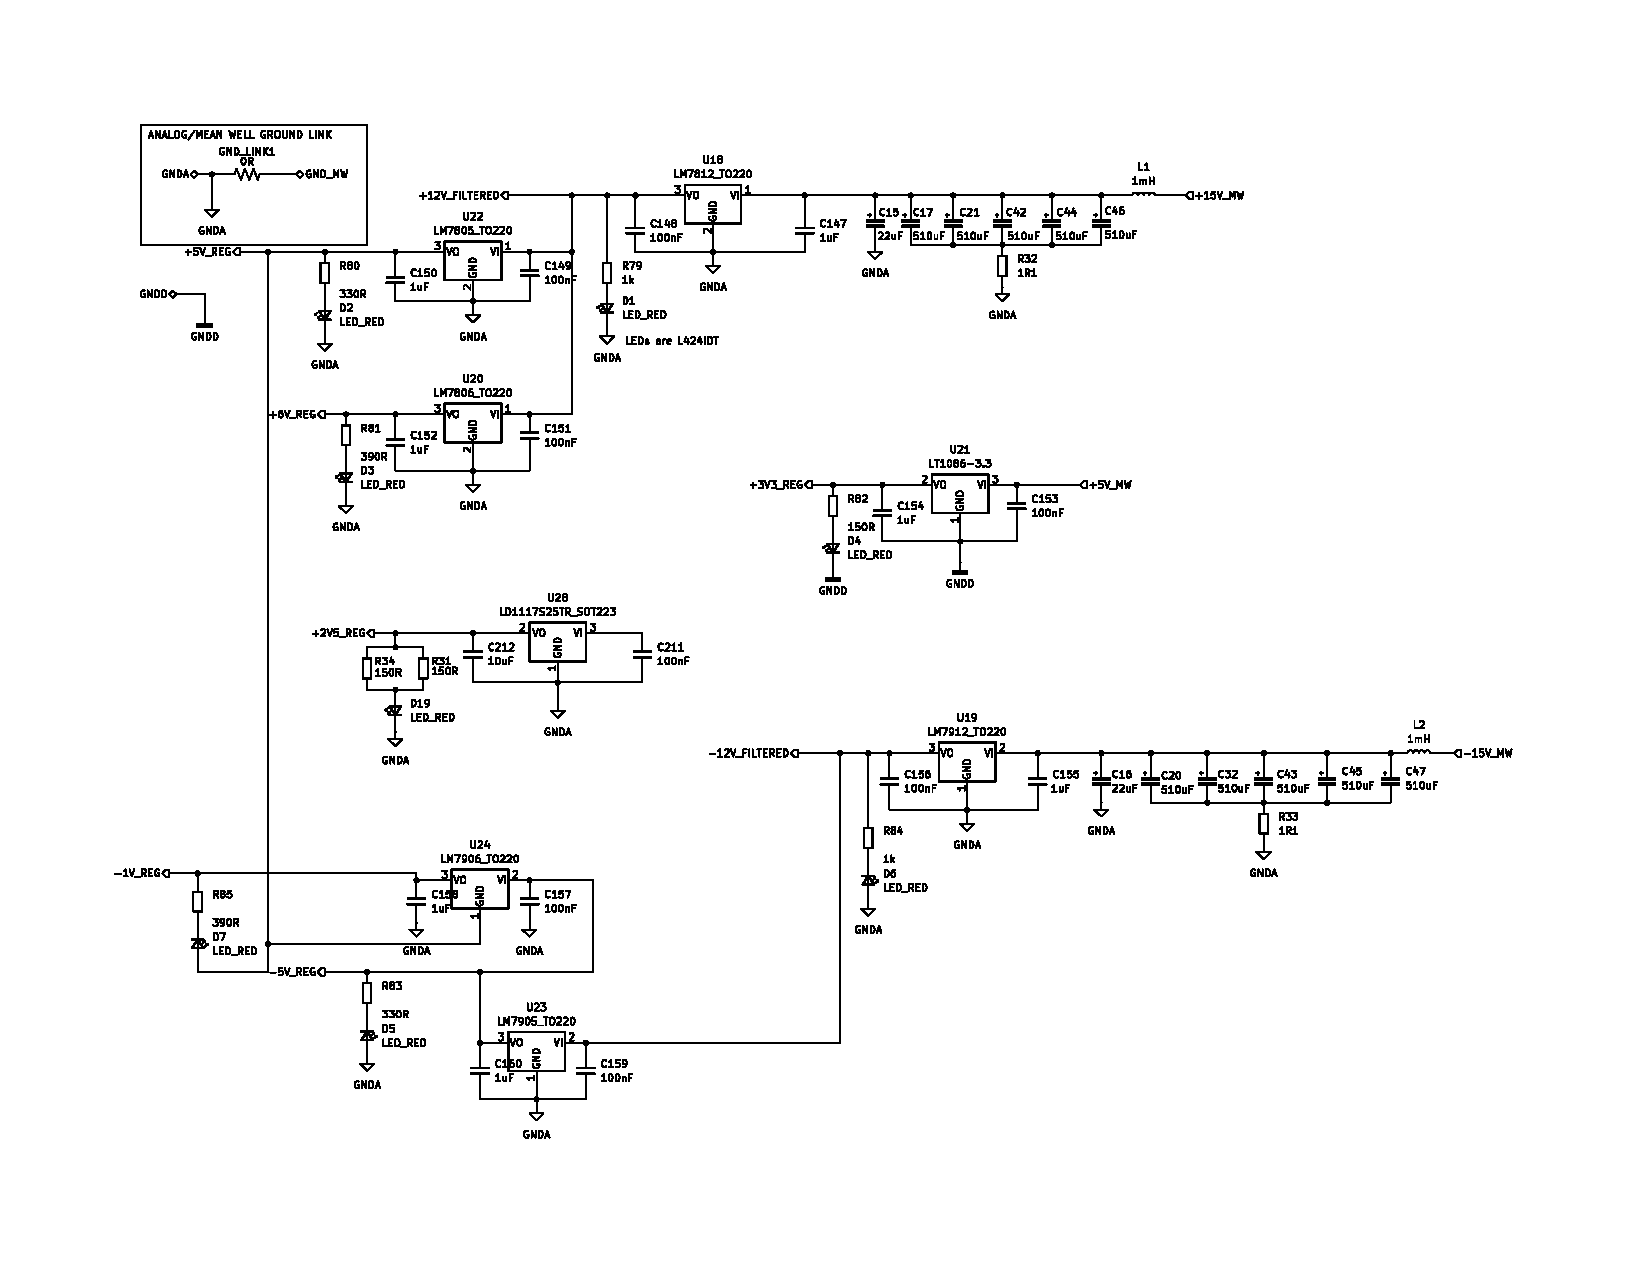
\includegraphics[clip, trim=0 50 0 0, width=1\textwidth]{Appendix/Figures/A_SCH_DCSUPPLY.pdf}
    \caption{The schematic for the DC supplies. The Mean Well RT65C external power supply is not shown on this schematic, but the nets marked with \_MW are inputs from this RT65C. All the DC supplies in table \refq{tab:7_1_6_Supply_Voltages} are set by fixed voltage regulators.}
    \label{fig_7_1_6_DCSUPPLY}
\end{figure}

Note how on figure \refq{fig_7_1_6_DCSUPPLY} there are two 'GNDx' nets, one is marked GNDA and the other GNDD. This is to keep the analog and digital grounds separated when making the board layout. The two nets will be joined together in a single point with the 'GND\_LINK' component in the upper left corner, this will be described more in section \refq{subsec:PCBDesign}.

As can be seen on figure \refq{fig_7_1_6_DCSUPPLY} the \SIQ{-1}{\volt} supply is generated by setting the ground reference of a LM7906 \SIQ{-6}{\volt} regulator to \SIQ{+5}{\volt} this is because no fixed \SIQ{-1}{\volt} regulator was available. Shifting the ground reference by \SIQ{+5}{\volt} will cause the output of the \SIQ{-6}{\volt} regulator to be \SIQ{-1}{\volt}.

Each of these regulators have a minimum load requirement in order to function correctly and the forward current for each of the red LEDs on figure \refq{fig_7_1_6_DCSUPPLY} have been chosen to provide the minimum load. The voltage regulators for the analog front end are all tapped from the output of the $\pm 12V$ regulators, which will see the highest load. Using table \refq{tab:total_power_current}, in appendix \refq{App:PowerConsumption}, the 12V regulator will see a current draw of $I_L = 265e-3$ and dissipate \SIQ{795}{\milli\watt} as shown in eq \refq{eq:7_1_6_PD12}.

\begin{equation}\label{eq:7_1_6_PD12}
    P_{D12V} = (V_{MW} - V_O) \cdot I_L = (15 - 12)\cdot 265e-3 = 795e-3
\end{equation}

The LM7812 regulator comes in a TO-220 package with a junction-to-ambient thermal resistance of \SIQ{23.9}{\degree}/W and will reach a junction temperature of \SIQ{44}{\degree}C as shown in eq \refq{eq:7_1_6_T12V} assuming an ambient temperature of \SIQ{25}{\degree}C

\begin{equation}\label{eq:7_1_6_T12V}
    T_{12V} = P_(D12V) \cdot R_{JA} + T_A = 795e-3 \cdot 23.9 + 25 = 44
\end{equation}

The 5V regulator will see an estimated load of $I_{L5V} = 198e-3$ and will dissipate more power as it causes a significant voltage drop. The power dissipated in this regulator is \refq{eq:7_1_6_PD5V}
\begin{equation}\label{eq:7_1_6_PD5V}
    P_{D5V} = (V_{12} - V_O) \cdot I_L = (12 - 5)\cdot 198e-3 = 1386e-3
\end{equation}

The 5V regulator is, also, in a TO-220 package and will reach a junction temperature of \SIQ{58.12}{\degree}C as shown in equation \refq{eq:7_1_6_T5V}.

\begin{equation}\label{eq:7_1_6_T5V}
    T_{5V} = P_{D5V} \cdot  R_{JA} + 25 = 1386e-3 \cdot 23.9 + 25  = 58.12
\end{equation}

Neither of these temperatures are close to the recommended maximum junction temperature of \SIQ{125}{\degree}C. This is acceptable and provides a large margin for error in the estimated load. The negative supply rails has a similar load and will reach similar junction temperatures.


